\section{Binomial model}
\label{sec:binomial_tree}
This section generalizes the numerical illustration of the binomial model for the option value given in Section \ref{sec:intro_binomial_model}. Then, further applications of the binomial model are presented. The content of this section is heavily based on Chapter 3 of \cite{pw_iqf2ed_2007} and Chapter 10 of \cite{pw_mathfinderiv_1995}. It is worth to repeat the Paul Wilmott's comment on the binomial model that ``the binomial model is great for getting intuition about delta hedging and risk-neutral pricing but not for real-life pricing''.


\subsection{Initiation}
In the binomial model, we assume that the asset, which initially has the value $S$, can, during a time step $\delta t$, either:
\begin{itemize}
    \setlength\itemsep{0em}
    \item rise or fall to a value $u \times S$ or $v \times S$, respectively with $0 < v < 1 < u$;
    \item the probability of a rise is $p$ and so the probability of a fall is $1-p$;
    \item the three constants $(u,v,p)$ are chosen to give the binomial walk the same characteristics as the asset we are modeling.
\end{itemize}

For a more proper approach to quantitative finance, instead of using $(u,v,p)$, we write everything in terms of the mean and the standard deviation of the random walk. That involves writing $(u,v,p)$ in terms of what are known as the drift and the volatility of the asset, the drift $\mu$ is the average rate at which the asset rises, and the volatility $\sigma$ is a measure of its randomness. Since we have three parameters to choose $(u,v,p)$ and only two statistical quantities to fit $(\mu,\sigma)$, choices for conversion is unlimited. One of the possible conversion follows:
\begin{align}
    u &= 1 + \sigma \sqrt{\delta t} \\
    v &= 1 - \sigma \sqrt{\delta t} \\
    p &= \frac{1}{2} + \frac{\mu \sqrt{\delta t}}{2 \sigma}    
\end{align}
This conversion will be described in a little bit more details in the next section. The correction of this conversion is, however, examined below.

The expected asset price after one time step is:
\begin{align}
    p u S + (1-p) v S &= \left( \frac{1}{2} + \frac{\mu \sqrt{\delta t}}{2 \sigma} \right) \left( 1 + \sigma \sqrt{\delta t} \right) S + \left( \frac{1}{2} - \frac{\mu \sqrt{\delta t}}{2 \sigma} \right) \left( 1 - \sigma \sqrt{\delta t} \right) \\
                      &= \left( 1 + \mu \delta t \right) S
\end{align}
so the expected change in the asset is $\mu S \delta t$. Because the expected return is $\mu \delta t$ so the expected asset price is corrected.

The variation of change in the asset price is:
\begin{align}
    S^2 &\left( p(u - 1 - \mu \delta t)^2 + (1-p)(v - 1 - \mu \delta t)^2 \right) \\
     &= S^2 \left( \left( \frac{1}{2} + \frac{\mu \sqrt{\delta t}}{2 \sigma} \right) \left( \sigma \sqrt(\delta t) - \mu \delta t \right)^2 + \left( \frac{1}{2} - \frac{\mu \sqrt{\delta t}}{2 \sigma} \right) \left( \sigma \sqrt(\delta t) + \mu \delta t \right)^2 \right) \\
     &= S^2 \left( \sigma^2 \delta t - \mu^2 \delta t^2 \right)
\end{align}
so the standard deviation of asset changes is (approximately) $S \sigma \sqrt{\delta t}$. Because the standard deviation of return is $\sigma \sqrt{\delta t}$ so the standard deviation of asset changes is corrected.

Because of the similarity in the expected change in the asset and the standard deviation of asset changes, it can be concluded that the conversion from $(u,v,p)$ to $(\mu,\sigma)$ is acceptable.



\subsection{Value of an option}
This section is a numerical generalization of Section \ref{sec:intro_binomial_model}. Suppose that we have an underlying asset of value $S$, and we know the value of the option at time $t + \delta t$. Now construct a portfolio at time $t$ consisting of one option and a short position in a quantity $\Delta$ of the underlying. 

At time $t$ this portfolio has value:
\begin{equation}
    \Pi = V - \Delta S
\end{equation}
where the option value $V$ is, for the moment, unknown. At time $t + \delta t$, the option takes one of two values depending on whether the asset rises or falls:
\begin{equation}
    V^+ \quad \text{or} \quad V^-
\end{equation}
and hence, the portfolio becomes either:
\begin{equation}
    V^+ - \Delta u S \quad \text{or} \quad V^- - \Delta u S
\end{equation}
Because we know $V^+, V^-, u, v, S$, the values of both expressions are just linear functions of $\Delta$.



\subsubsection{Hedging}
Having the freedom to choose $\Delta$, we can make the value of this portfolio the same whether the asset rises or falls, i.e. hedging, which means:
\begin{equation}
    V^+ - \Delta u S = V^- - \Delta u S
\end{equation}
by choosing:
\begin{equation}
    \Delta = \frac{V^+ - V^-}{(u-v) \times S}
\end{equation}

The portfolio value is then:
\begin{equation}
    V^+ - \Delta u S = V^+ - \frac{u(V^+ - V^-)}{u-v}
\end{equation}
if the stock rises; or:
\begin{equation}
    V^- - \Delta u S = V^- - \frac{v(V^+ - V^-)}{u-v}
\end{equation}
if the stock falls. And, of course, these two expressions are the same.



\subsubsection{No arbitrage}
Since the value of the portfolio is guaranteed, following the no-arbitrage argument, its value must coincide with the value of the original portfolio plus any interest earned at the risk-free rate. Let's denote the portfolio value by:
\begin{equation}
    \Pi + \delta \Pi
\end{equation}
which just means the original portfolio value plus the change in value. Thus:
\begin{equation}
    \delta \Pi = r \Pi \delta t
\end{equation}

The full formulation for the portfolio value is then:
\begin{equation}
    \Pi + \delta \Pi = \Pi + r \Pi \delta t = \Pi (1 + r \delta t) = V^+ - \frac{u(V^+ - V^-)}{u-v}
\end{equation}
with:
\begin{equation}
    \Pi = V - \Delta S = V - \frac{V^+ - V^-}{u-v}
\end{equation}
Rearrange the above two equations as an equation for $V$ we get:
\begin{equation}
    (1 + r \delta t)V = (1 + r \delta t) \frac{V^+ - V^-}{u-v} + \frac{uV^- - vV^+}{u-v}
\end{equation}
This is an equation for $V$ given $V^+$ and $V^-$ - the option values at the next time step, and the parameters $u$ and $v$ describing the random walk of the asset. 

This equation can also be written in the more compacted form:
\begin{equation}
    V = \frac{1}{1 + r \delta t} \left( p' V^+ + (1-p')V^- \right)
    \label{equ:option_value_binomial}
\end{equation}
in which:
\begin{equation}
    p' = \frac{1}{2} + \frac{r \sqrt{\delta t}}{2 \sigma}
\end{equation}.
The right-hand side of Equation \ref{equ:option_value_binomial} is just like a discounted expectation. The terms in the parentheses are the sum of probabilities multiplied by events. The probability $p'$ is called the \textbf{risk-neutral probability}. It is like the real probability but used in the \textbf{risk-free world}. In the real world, the probability is calculated with the drift $\mu$ instead of the interest rate $r$:
\begin{equation}
    p' = \frac{1}{2} + \frac{r \sqrt{\delta t}}{2 \sigma} \quad \text{vs.} \quad p = \frac{1}{2} + \frac{\mu \sqrt{\delta t}}{2 \sigma} 
\end{equation}. 
Observe that the risk-free interest rate $r$ plays two roles in option valuation. It's used once for discounting to give present value, and it's used as the drift rate in the risk-neutral asset price random walk.

Equation \ref{equ:option_value_binomial} is equivalent to the statement ``the option value at any time is the present value of the risk-neutral expected value at any later time'', so it is actually the risk-neutral expectation.



\subsubsection{Binomial tree}
The binomial tree presents the possible development of the asset value following the random walk of the binomial model all the way until expiry. An example of the binomial tree is given in Figure \ref{fig:binomial_math} where the nodes represent the values taken by the asset. Observe how the tree bends due to the geometric nature of the asset growth although it is normally presented in an equal-distance manner as in Figure \ref{fig:binomial_tree_general}. 

\begin{figure}[H]
    \centering
    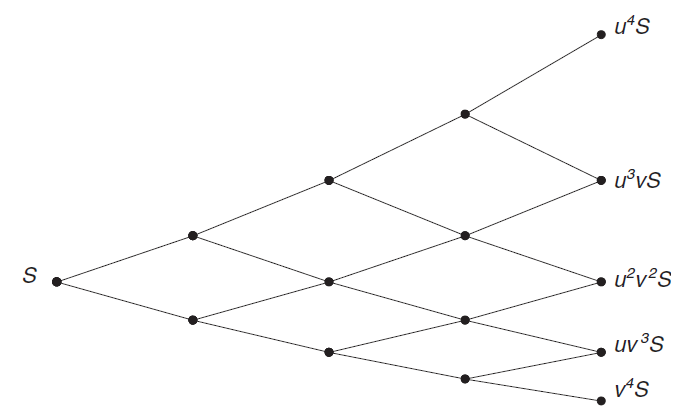
\includegraphics[width=0.6\textwidth]{figure/binomial_math.png}
    \caption{A binomial tree}
    \label{fig:binomial_math}
\end{figure}

The probability of reaching a particular node in the binomial tree depends on the number of distinct paths to that node and the probabilities of the up and down moves. The binomial tree therefore contains within it an approximation to the probability density function for the lognormal random walk, Figure \ref{fig:binomial_tree_general}.

\begin{figure}[H]
    \centering
    \begin{subfigure}[b]{0.4\textwidth}
        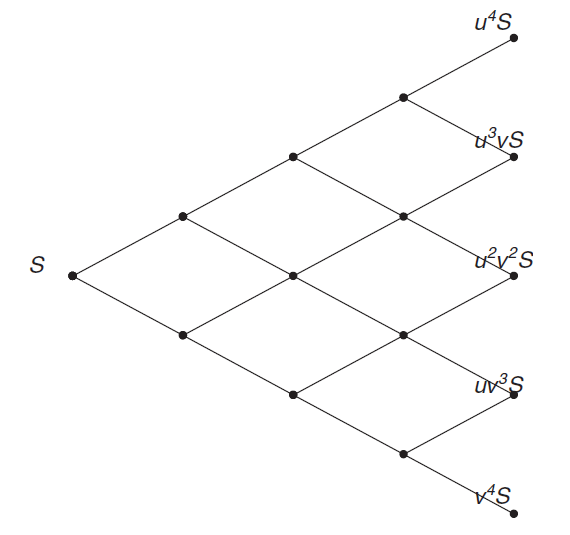
\includegraphics[width=\textwidth]{figure/binomial_schematic.png}
        \caption{Schematic presentation}
    \end{subfigure}
    \begin{subfigure}[b]{0.4\textwidth}
        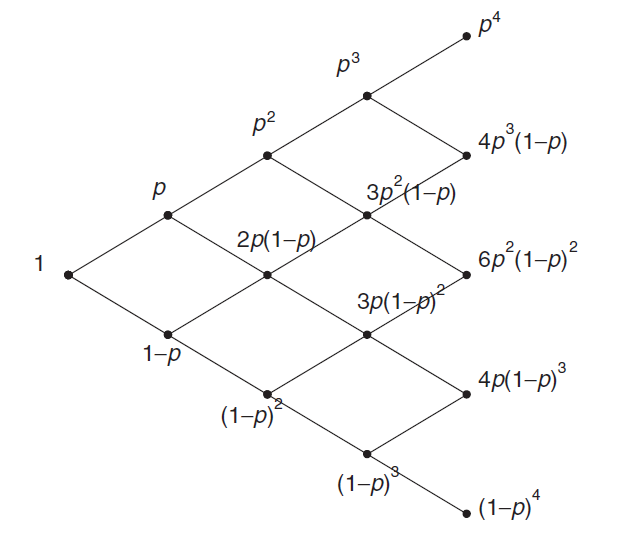
\includegraphics[width=\textwidth]{figure/binomial_counting.png}
        \caption{Counting path - Probability}
    \end{subfigure}
    \caption{A binomial tree}
    \label{fig:binomial_tree_general}
\end{figure}



\subsubsection{The Greeks}
The greeks are defined as derivatives of the option value with respect to various variables and parameters. It is important to distinguish whether the differentiation is with respect to a variable or a parameter. If the differentiation is only with
respect to the asset price and/or time then there is sufficient information in our binomial tree to estimate the derivative. It may not be an accurate estimate, but it will be an estimate. The option's $\Delta$, $\Gamma$ and $\Theta$ can all be estimated from the tree. On the other hand, it is harder if you want to examine the sensitivity of the option with respect to one of the parameters. They are harder to calculate in the sense that you must perform a second binomial calculation. This applies to the option's Vega and $\rho$.

The option's delta is defined by:
\begin{equation}
    \Delta = \frac{V^+ - V^-}{(u-v) \times S}
\end{equation}
As all quantities on the right-hand side are known, we can calculate the delta directly from the tree. In the limit as the time step approaches zero, the delta becomes:
\begin{equation}
    \Delta = \frac{\partial V}{\partial S}
\end{equation}

The gamma of the option is also defined as a derivative of the option with respect to the underlying:
\begin{equation}
    \Gamma = \frac{\partial^2 V}{\partial S^2}
\end{equation}
Gamma is a measure of how much we must rehedge at the next time step. Using the binomial tree, the gamma is just the change in the delta from one of these to the other divided by the distance between them. It, however, will be much easier when we use a finite-difference grid to estimate this quantity.

The theta of the option is the sensitivity of the option price to time, assuming that the asset price does not change. Again, this is easier to calculate from a finite difference grid. An obvious choice for the discrete time definition of theta is to interpolate between $V^+$ and $V^-$ to find a theoretical option value had the asset not changed and use this to estimate:
\begin{equation}
    \Gamma = \frac{\partial V}{\partial t}
\end{equation}
which results in:
\begin{equation}
    \Gamma = \frac{\frac{1}{2} \left( V^+ - V^- \right)}{\delta t}
\end{equation}

Estimating the other type of greeks, the ones involving differentiation with respect to parameters, requires performing a second binomial calculation. The calculation of the option's vega is presented here for illustration. The vega is the sensitivity of the option value to the volatility:
\begin{equation}
    \text{Vega} = \frac{\partial V}{\partial \sigma}
\end{equation}
Suppose we want to find the option value and the vega when the volatility is 20\%. The most efficient way to do this is to calculate the option price twice, using a binomial tree, with two different values of $\sigma$. Calculate the option value using a volatility of $\sigma \pm \varepsilon$, for a small number $\varepsilon$; call the values you find $V_\pm$. The option value is approximated by the average value:
\begin{equation}
    V = \frac{1}{2} \left( V_{+} - V_{-} \right)
\end{equation}
and the vega is approximated by:
\begin{equation}
    \text{Vega} = \frac{V_{+} - V_{-}}{2 \varepsilon}
\end{equation}
The idea can be applied to other greeks.



\subsection{Implementation}
\subsubsection{$(u,v,p)$ to $(\mu,\sigma)$}
The three constants $(u,v,p)$ are chosen to give the binomial walk the same drift and standard deviation $(\mu,\sigma)$ as the stock we are trying to model. Our starting point, the lognormal random walk
\begin{equation}
    dS = \mu \; S \; dt + \sigma \; S \; dX
\end{equation}
has the solution:
\begin{equation}
    S(t) = S(0) e^{\left( \mu - \frac{1}{2} \sigma^2 \right) t + \sigma \phi \sqrt{t}}
\end{equation}
where $\phi$ is a standardized normal random variable. 

For the binomial random walk to have the correct drift over a time period of $\delta t$ we need (details can be found in \cite{pw_mathfinderiv_1995}):
\begin{equation}
    puS + (1-p)vS = S \times E \left[ e^{\left( \mu - \frac{1}{2} \sigma^2 \right) \delta t + \sigma \phi \sqrt{\delta t}} \right] = S \times e^{\mu \delta t}
\end{equation}
i.e.
\begin{equation}
    pu + (1-p)v = e^{\mu \delta t}
\end{equation}
Rearranging this equation gives us:
\begin{equation}
    p = \frac{e^{\mu \delta t} - v}{u - v}
    \label{equ:binomial_cond_1}
\end{equation}

For the binomial random walk to have the correct variance we need (details can be found in \cite{pw_mathfinderiv_1995}):
\begin{equation}
    pu^2 + (1-p)v^2 = e^{\left( 2\mu + \sigma^2 \right)\delta t}
    \label{equ:binomial_cond_2}
\end{equation}

Having only two equations for the three parameters gives us one degree of freedom in this choice. As Equations \ref{equ:binomial_cond_1} and \ref{equ:binomial_cond_2} determine all the statistically important properties of the discrete random walk, the choice of the third equation is somewhat arbitrary. This degree of freedom is often used to give the random walk the further property that after an up and a down movement (or a down followed by an up) the asset returns to its starting value $S$. This gives us the requirement that:
\begin{equation}
    v(uS) = u(vS) = S
\end{equation}
i.e. 
\begin{equation}
	uv = 1
	\label{equ:binomial_cond_3}
\end{equation}
This choice leads to a tree in which the starting asset price reoccurs every even time-step and which is symmetric about this price, Figure \ref{fig:binomial_tree_3rd}(a). Another popular choice is:
\begin{equation}
    p = \frac{1}{2}
\end{equation}
which leads to a tree oriented in the direction of the drift, Figure \ref{fig:binomial_tree_3rd}(b) since the probabilities of an up-jump and a down-jump are equal.

\begin{figure}[H]
    \centering
    \begin{subfigure}[b]{0.45\textwidth}
        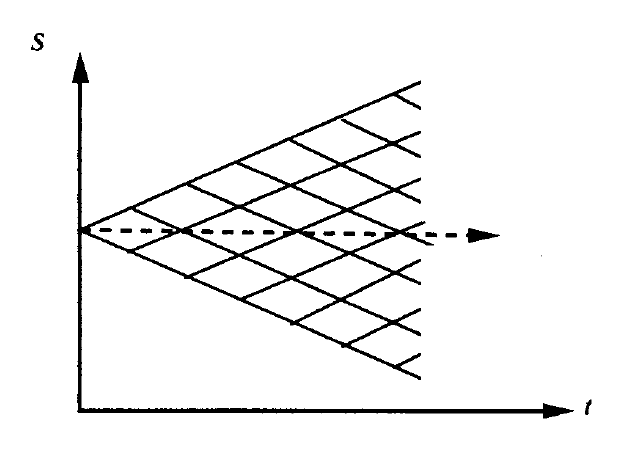
\includegraphics[width=\textwidth]{figure/uv=1.png}
        \caption{A tree with $u \times v = 1$}
    \end{subfigure}
    \begin{subfigure}[b]{0.45\textwidth}
        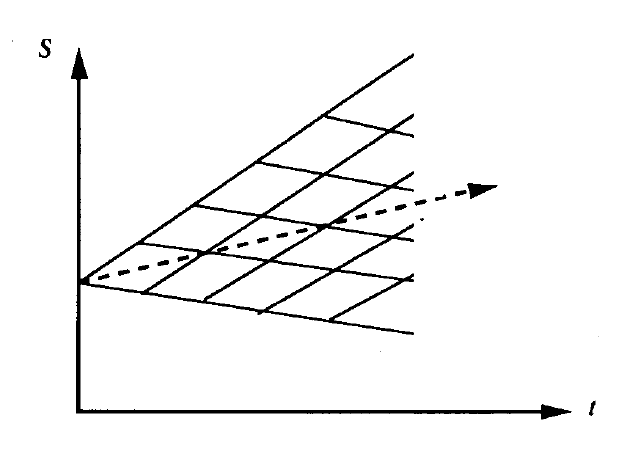
\includegraphics[width=\textwidth]{figure/p=05.png}
        \caption{A tree with $p = \frac{1}{2}$}
    \end{subfigure}
    \caption{Different binomial trees corresponding to the third equation}
    \label{fig:binomial_tree_3rd}
\end{figure}

This note only consider the first choice of freedome; correspondingly, Equations \ref{equ:binomial_cond_1}, \ref{equ:binomial_cond_2} and \ref{equ:binomial_cond_3} can be solved to give:
\begin{equation}
    u = \frac{1}{2} \left( e^{-\mu \delta t} + e^{\left( \mu + \sigma^2 \right)\delta t} \right) + \frac{1}{2} \sqrt{\left( e^{-\mu \delta t} + e^{\left( \mu + \sigma^2 \right)\delta t} \right)^2 - 4}
    \label{equ:binomial_u}
\end{equation}

The following approximations are good enough for most purposes:
\begin{align}
    u &\approx 1 + \sigma \delta t^{1/2} + \frac{1}{2} \sigma^2 \delta t \\
    v &\approx 1 - \sigma \delta t^{1/2} + \frac{1}{2} \sigma^2 \delta t \\
    p &\approx \frac{1}{2} + \frac{\left( \mu - \frac{1}{2} \sigma^2 \right) \delta t^{1/2}}{2 \sigma}
\end{align}

If the above derivation is being used for pricing options, the $\mu$ should be replaced by $r$ everywhere.



\subsubsection{Data structures}
The asset price and the option value are stored in two-dimensional array for clarity. The notation $S_i^n$ means the asset price at the $n$-th time step and at the node $i$ from the bottom, $0 \leq i \leq n$. In the lognormal model:
\begin{equation}
    S_i^n = S \times u^i v^{n-i}
\end{equation}
The notation $V_i^n$ means the option value at the same node. Our goal is to find $V_0^0$ knowing the payoff, i.e. knowing $V_i^N$ for all $0 \leq i \leq N$ where $N$ is the number of time steps. 


\subsubsection{Payoff function}
Assuming that we know the payoff function for our derivative security, and that it depends only on the values of the underlying asset at expiry, we are able to value it at expiry, i.e. time-step $N \delta t$.

If we are considering a put, we find that:
\begin{equation}
    V_i^N = \textbf{max} \left( E - S_i^N, 0 \right) \quad i = 0,1,2...,N
\end{equation}
where $E$ is the exercise price (strike). For a call, we find that:
\begin{equation}
    V_i^N = \textbf{max} \left( S_i^N - E, 0 \right) \quad i = 0,1,2...,N
\end{equation}



\subsubsection{Implementation}
The implementation is quite straight-forward for the European-style exercise. First, we build a tree of possible asset prices; then find the values of the option at expiry using the \textbf{payoff\_function}; finally, calculate the present values of the expected values of the option price under a risk-neutral random walk from expiry back until the present. The algorithm is presented below for the asset price $Asset$, the strike value $E$, the interest rate $r$, the volatility $\sigma$, the expiry $T$ and the number of time step $N$. The code can be found \href{https://github.com/chitn/quantfin_study/blob/master/code/binomial_model.py}{here}. 

\vspace{\baselineskip}
\begin{algorithm}[H]
\caption{European-style exercise}
\label{algo:binomial_european}  
\Begin{
    $Asset, E, r, \sigma, T, N $                      \tcc*[r]{Input} 
    \text{Time step     } $\delta t = \frac{T}{N}$    \tcc*[r]{Initialisation}
    \text{Discount rate } $dcr = \exp(-r \delta t)$                     \\
    \text{Calculate $(u, v, p)$ following \ref{equ:binomial_u}, \ref{equ:binomial_cond_3} and \ref{equ:binomial_cond_1}, respectively} \\
    \text{2D-array of asset value  $S = 0$ and option value $V = 0$}    \\
   
    \tcc*[r]{Calculate asset values}
    \text{Present asset price } $S_0^0 = Asset$  \\
    \For{i = 1 $\rightarrow$ N}{
        $S_0^i = S_0^{i-1} \times v$             \\
        \For{j = i $\rightarrow$ 1}{
            $S_j^i = S_{j-1}^{i-1} \times u$     \\
        }
    }       
    \tcc*[r]{Calculate option values}
    \For{i = 1 $\rightarrow$ N}{                 
         $V_i^N = \textbf{payoff\_function} \left(S_i^N, E\right)$  \\
    } 
    \For{i = N-1 $\rightarrow$ 0}{
        \For{j = 0 $\rightarrow$ i+1}{
            $V_j^i = \left( p \times V_{j+1}^{i+1} + (1-p) \times V_{j}^{i+1} \right) \times dcr$   
        }
    }    
    \text{Present option value } $Option = V_0^0$     
} 
\end{algorithm}
\vspace{\baselineskip}

The implementation for the American-style exercise is almost identical to that for the European-style exercise except a minor modification to address the early exercise to avoid arbitrage, i.e. the option value should be larger or equal to the payoff at any time. If our theoretical value calculated following \ref{equ:option_value_binomial} falls below the payoff then it is time to exercise. 
\begin{equation}
    V_j^i = \textbf{max} \left( \frac{p \times V_{j+1}^{i+1} + (1-p) \times V_{j}^{i+1}}{\exp(r \delta t)},
\textbf{payoff\_function} \left(S_j^i, E\right) \right)
\end{equation}
The algorithm for the American-style exercise is then only different from Algorithm \ref{algo:binomial_european} in calculating the intermediate option values, i.e. the option values is calculated by taking the maximum of the expected values and the payoff for early exercise at each time-step and the asset price.

\vspace{\baselineskip}
\begin{algorithm}[H]
\caption{American-style exercise}
\Begin{
    \For{i = N-1 $\rightarrow$ 0}{
        \For{j = 0 $\rightarrow$ i+1}{
            $\text{Theoretical option value } tv = \left( p \times V_{j+1}^{i+1} + (1-p) \times V_{j}^{i+1} \right) \times dcr $ \\
            $\text{Early exerice value } ev = \textbf{payoff\_function} \left(S_j^i, E\right) $                                  \\
            $V_j^i = \textbf{max} \left( tv, ev \right)$   
        }
    }    
    \text{Present option value } $Option = V_0^0$     
}
\label{algo:binomial_american}   
\end{algorithm}
\vspace{\baselineskip}

Figure \ref{fig:binomial_euam_put} illustrate the option value for European- and American-put options corresponding to different numbers of time steps $N$. The input is as follows $Asset = 100, E = 110, r = 0.06, \sigma = 0.3, T = 0.25 \& 1 \text{ (3-month and 1-year duration)}$.

\begin{figure}[H]
    \centering
    \begin{subfigure}[b]{0.45\textwidth}
        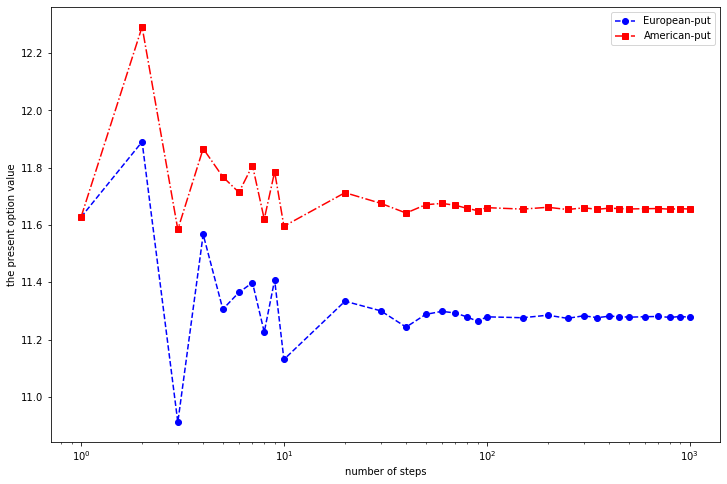
\includegraphics[width=\textwidth]{figure/binomial_model_euam_put_025.png}
        \caption{Expiry in 3-month}
    \end{subfigure}
    \begin{subfigure}[b]{0.45\textwidth}
        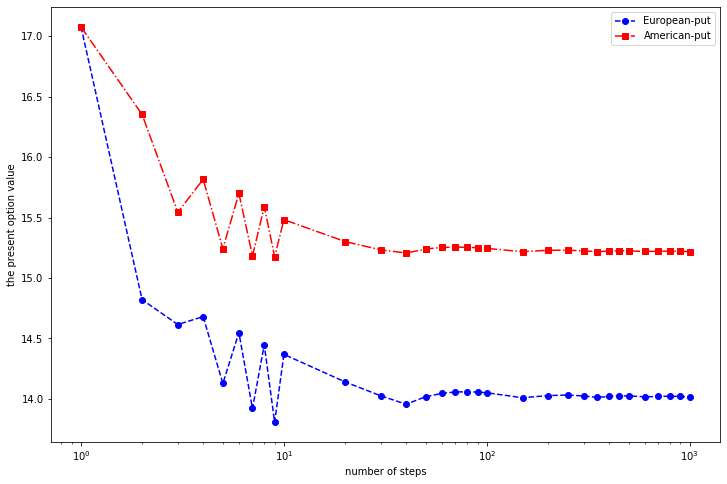
\includegraphics[width=\textwidth]{figure/binomial_model_euam_put_100.png}
        \caption{Expiry in 1-year}
    \end{subfigure}
    \caption{Binomial model for European- and American-put options}
    \label{fig:binomial_euam_put}
\end{figure}



\subsubsection{Dividend yields}
The binomial model can easily accommodate a constant dividend yield $D_0$ paid on the underlying. The effective risk-free growth rate of the asset becomes $\mu - D_0$ instead of $\mu$, that is:
\begin{equation}
    dS = \left( \mu - D_0 \right) \; S \; dt + \sigma \; S \; dX
\end{equation}
therefore we should replace $\mu$ by $\mu - D_0$ in the derivation of $(u,v,p)$. For the case $uv = 1$, the formulations of $(u,v,p)$ become:
\begin{align}
    A &= \frac{1}{2} \left( e^{-\left( \mu - D_0 \right) \delta t} + e^{\left( \mu - D_0 + \sigma^2 \right)\delta t} \right) \\
    u &= A + \sqrt{A^2 - 1} \\
    v &= A - \sqrt{A^2 - 1} \\
    p &= \frac{e^{\left( \mu - D_0 \right) \delta t} - v}{u - v}
\end{align}

The only effect of continuous dividend yields is to modify the probability $p$ and the jump sizes $u$ and $v$. Therefore, the same algorithm given in the previous section for both the European- and American-option values can still be used by simply modifying the parameters $(u,v,p)$ according to the above equations. 


\subsection{Continuous-time limit}
The binomial model is a discrete-time model for the option pricing. From this model, we can develop a continuous-time model (the famous Black-Scholes model) by let $\delta t \rightarrow 0$. 

We will start with the three approximation:
\begin{align*}
    u &\approx 1 + \sigma \sqrt{\delta t} \\
    v &\approx 1 - \sigma \sqrt{\delta t} \\
    p &\approx \frac{1}{2} + \frac{\mu \sqrt{\delta t}}{2 \sigma}    
\end{align*}
as introduced at the beginning of this section.

Next, we write:
\begin{align}
    V   &= V(S , t)                                          \\
    V^+ &= V(uS, t + \delta t) = V(S + (u-1)S, t + \delta t) \\
    V^- &= V(vS, t + \delta t) = V(S + (v-1)S, t + \delta t)   
\end{align}
and apply the Taylor series approximation with small $\delta t$ for $V^+$ and $V^-$ following:
\begin{equation}
    V(S + \delta S, t + \delta t) \approx V(S,t) + \delta t \frac{\partial V}{\partial t} + \delta S \frac{\partial V}{\partial S} + \frac{1}{2} \delta S^2 \frac{\partial^2 V}{\partial S^2} + ...
\end{equation}
This series goes on for ever, but we only use the largest and most important terms, those which are required for the Black–Scholes analysis.

By substituting $V^+$ and $V^-$ into the equation:
\begin{equation*}
    \Delta = \frac{V^+ - V^-}{(u-v) \times S}
\end{equation*}
to achieve:
\begin{equation}
    \Delta \approx \frac{\partial V}{\partial S} \quad \text{as } \delta t \rightarrow 0
\end{equation}

Then, by substituting $V$, $V^+$ and $V^-$ into the equation:
\begin{equation*}
    \left( 1 + r \delta t \right) V = p V^+ + (1-p)V^-
\end{equation*}
to find:
\begin{equation}
    \frac{\partial V}{\partial t} + \frac{1}{2} \sigma^2 S^2 \frac{\partial^2 V}{\partial S^2} + rS \frac{\partial V}{\partial S} - rV = 0
\end{equation}
This is the Black–Scholes equation. Again, the drift rate $\mu$ has disappeared from the equation. 

The famous Black–Scholes equation will be derived later using stochastic calculus rather than via the binomial model. The stochastic calculus derivation is far more useful than the binomial and being far easier to generalize.



\subsection{Miscellaneous \textcolor{red}{[FUTURE]}}
\begin{itemize}
    \setlength\itemsep{0em}
    \item Replicating portfolio
    \item Asset price process
\end{itemize}



